\chapter{Versuch 6: Aktiver Tiefpass erster Ordnung}

\section{Einleitung}

In diesem Versuch wird ein aktiver Tiefpass erster Ordnung untersucht. 
Der aktive Tiefpass erster Ordnung besteht aus einem Operationsverstärker
und einem RC-Glied. 
Ziel des Versuchs ist es, die frequenzabhängige Verstärkung eines aktiven
Tiefpasses erster Ordnung zu bestimmen.

\section{Vorbereitung}

\subsection{Benötigte Geräte}

\begin{tabular}[h]{c|c}
    Widerstand 1 k$\Omega$ & 2\\
    \hline
    Widerstand 10 k$\Omega$ & 1\\
    \hline
    Operationsverstärker & \\
    \hline
    Netzgerät & Tenma 72-10495 Digital Control DC Power Supply\\
    \hline
    Funktionsgenerator & T3AFG80\\
    \hline
    Oszilloskop & Keysight DSOX1102A
    \label{tab:Versuch 6: Geräte}
\end{tabular}
\subsection{Schaltungsskizze}

Der Operationsverstärker wird als invertierender
Verstärker verwendet. Die Spannung u\textsubscript{e} wird an den
invertierenden Eingang des Operationsverstärkers angelegt. Die Ausgangsspannung
u\textsubscript{a} wird am Ausgang des Operationsverstärkers abgegriffen.

Die Schaltungsskizze sieht folgendermaßen aus:

\begin{figure}[H]
    \centering
    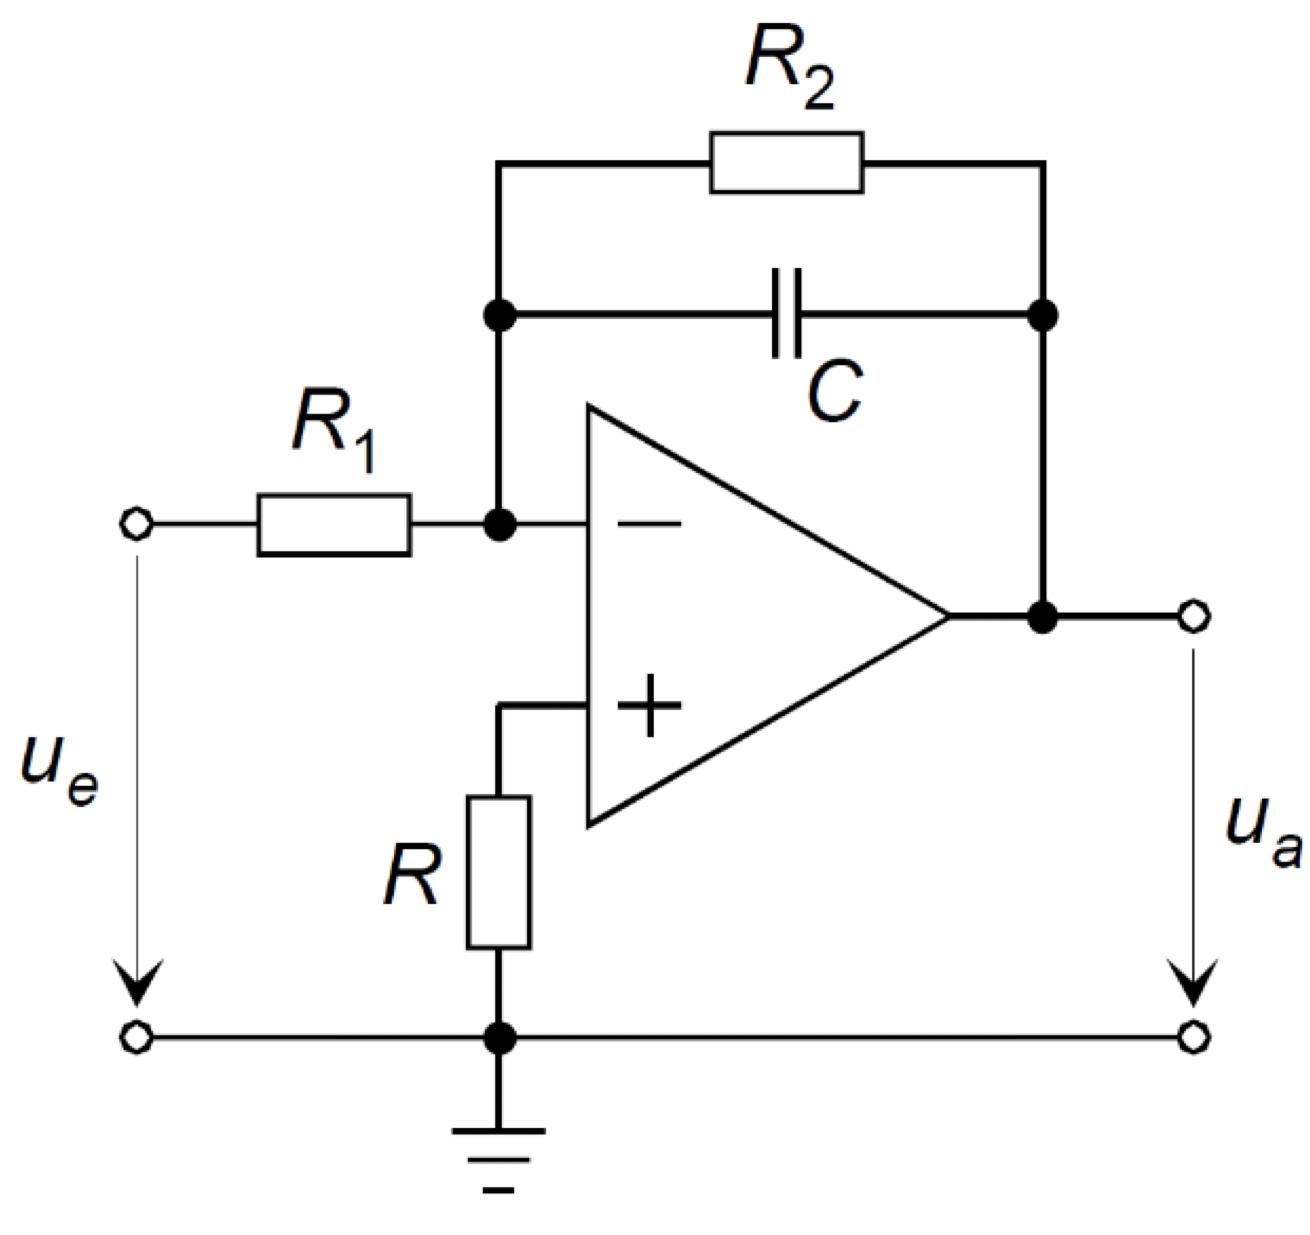
\includegraphics[height=7cm]{images/Versuch6/Schaltungsskizze.jpeg} 
    \caption{Schaltungsskizze}
    \label{fig: Schaltungsskizze}
\end{figure}


Die Verwendung des Widerstands R dient der Offset-Kompensation, 
um die Offset-Spannung des Operationsverstärkers auszugleichen. 
Diese Offset-Spannung stellt einen unvermeidlichen systematischen 
Fehler dar, der auftritt, wenn beide Eingänge des Operationsverstärkers
auf Masse gelegt sind. In solchen Fällen fließt ein geringer Strom 
durch die Widerstände 1 und 2, was dazu führt, dass das Potential 
des invertierenden Eingangs und des nicht-invertierenden Eingangs 
nicht mehr gleich ist. Dies wiederum erzeugt die Offset-Spannung.

\[
    R = R_2 || R_1 = \frac{R_1 \cdot R_2}{R_1 + R_2} = \frac{1k\Omega \cdot 10k\Omega}{1k\Omega + 10k\Omega} = 0.909 k\Omega
\]

In den meisten Schaltungsanalysen kann der Widerstand vernachlässigt 
werden, da der Eingangsstrom des Operationsverstärkers normalerweise 
sehr gering ist, und der invertierende Eingang nur selten auf Masse 
gelegt wird. Daher hat der Widerstand in der Regel keinen signifikanten
Einfluss auf die Funktion des Operationsverstärkers.

Gegebene Größen sind R\textsubscript{1} = 1k$\Omega$,
R\textsubscript{2} = 10k$\Omega$ und C = 10nF.
Des Weiteren ist u\textsubscript{e} als Sinusfunktion mit einer
Amplitude von 15V gegeben.
Als Näherung hierfür wird für R ein Widerstand der Größe
R\textsubscript{1} eingebaut. 

\subsection{Berechnung der Spannungsverstärkung}

Zur Berechnung der Spannungsverstärkung A\textsubscript{V} als
Funktion der Sinusfrequenz f wird folgende Formel benötigt:

\begin{equation}
    A\textsubscript{V} = -\frac{R_2}{R_1} \cdot \frac{1}{1 + j \cdot 2 \pi \cdot f \cdot R_2 \cdot C}
    \label{eq:AV}
\end{equation}

Für die Ausgangsspannung u\textsubscript{a} gilt also:
\begin{equation}
    u\textsubscript{a} = -A\textsubscript{V} \cdot u\textsubscript{e} = -\frac{R_2}{R_1} \cdot \frac{1}{1 + j 2 \pi f R_2 C} \cdot u\textsubscript{e}
    \label{eq:AV}
\end{equation}

Somit lässt sich die Funktion der Schaltung als frequenzabhängig beschreiben.
Bei niedrigen Frequenzen ist die Verstärkung $A\textsubscript{V}$ groß,
da der Kondensator als eine Unterbrechung wirkt. Bei hohen Frequenzen
ist der paralle Widerstand R\textsubscript{2} zu vernachlässigen und
die Schaltung verhält sich wie ein Integrator.


Messbar ist nur der reele Betrag der Spannungsverstärkung  
$|A\textsubscript{V}| = \sqrt{A\textsubscript{V} \cdot (A\textsubscript{V})^{*}} $.
Im folgenden wird gezeigt, dass es
\begin{equation}
    |A\textsubscript{V}| = C_1\frac{1}{\sqrt{1 + C_2(f)}}
    \label{eq:AV2}
\end{equation} 
gilt. Dafür wird zunächst 
$|A\textsubscript{V}|$ berechnet:

\[
    \begin{aligned}
    |A_V| & = \sqrt{\frac{R_2^2}{R_1^2} \cdot \frac{1}{1 + j 2 \pi f R_2 C} \cdot \frac{1}{1 + j 2 \pi f R_2 C}}
    = \frac{R_2}{R_1} \cdot \sqrt{\frac{1}{(1 + j 2 \pi f R_2 C) \cdot (1 + j 2 \pi f R_2 C)}} \\
    & = \frac{R_2}{R_1} \cdot \sqrt{\frac{1}{(1 - j 2 \pi f R_2 C + j 2 \pi f R_2 C - j^2 4 \pi^2 f^2 R_2 ^ 2 C^2)}}
    = \frac{R_2}{R_1} \cdot \frac{1}{\sqrt{1 + 4 \pi^2 f^2 R_2 ^ 2 C^2}} \\
    \end{aligned}
\]

Zusammenfassend gilt also:
\begin{equation}
    |A\textsubscript{V}| = \frac{R_2}{R_1} \cdot \frac{1}{\sqrt{1 + 4 \pi^2 f^2 R_2 ^ 2 C^2}}
    \label{eq:AV3}
\end{equation}

Nun werden $C_1$ und $C_2(f)$ aus \ref{eq:AV2} bestimmt: \par
Es gilt für $C_1$ = $\frac{R_2}{R_1}$,
 und für das frequenzabhängige $C_2(f)$ = $4 \pi^2 R_2 ^ 2 C^2$.

\subsection{Berechnung der Frequenzbereichen}
Um die Grenzfrequenz f\textsubscript{c} zu bestimmen, wird die
$C_2(f)$-Funktion gleich 1 gesetzt und nach f aufgelöst.

\[
    f_c = \sqrt{\frac{1}{4 \pi^2 R_2^2 C^2}} = \sqrt{\frac{1}{4 \pi^2 \cdot (10k\Omega)^2 \cdot (10nF)^2}} = 1591,549 Hz
\]

Die Frequenzen werden in drei Bereiche eingeteilt: \par

Frequenzbereich 1 FB1: $f \ll f_c$ 

\[
    |A_V| = \frac{R_2}{R_1} = \frac{}{} = 10
\]

Frequenzbereich 2 FB2: $ 0,25f_c < f < 4f_c$ \par
Untergrenze: 0,25f\textsubscript{c} = 397,887 Hz $\rightarrow$ $A_V = 9,7$ \par 
0,5f\textsubscript{c} = 795,774 Hz $\rightarrow$ $A_V = 8,9$ \par
2f\textsubscript{c} = 3183,096 Hz $\rightarrow$ $A_V = 4,5$ \par
Obergrenze: 4f\textsubscript{c} = 6366,196 Hz $\rightarrow$ $A_V = 2,4$ \par

Frequenzbereich 3 FB3: $f \gg f_c$ \par
\[
    |A_V| =\frac{1}{2 \pi f R_1 C} = \frac{1}{2 \pi \cdot 1k\Omega \cdot 10nF} = 15915,49 \frac{1}{F \Omega}\frac{1}{Hz}
\]  

Man zeichnet diese Werte in den Graphen:

\begin{figure}[H]
    \centering
    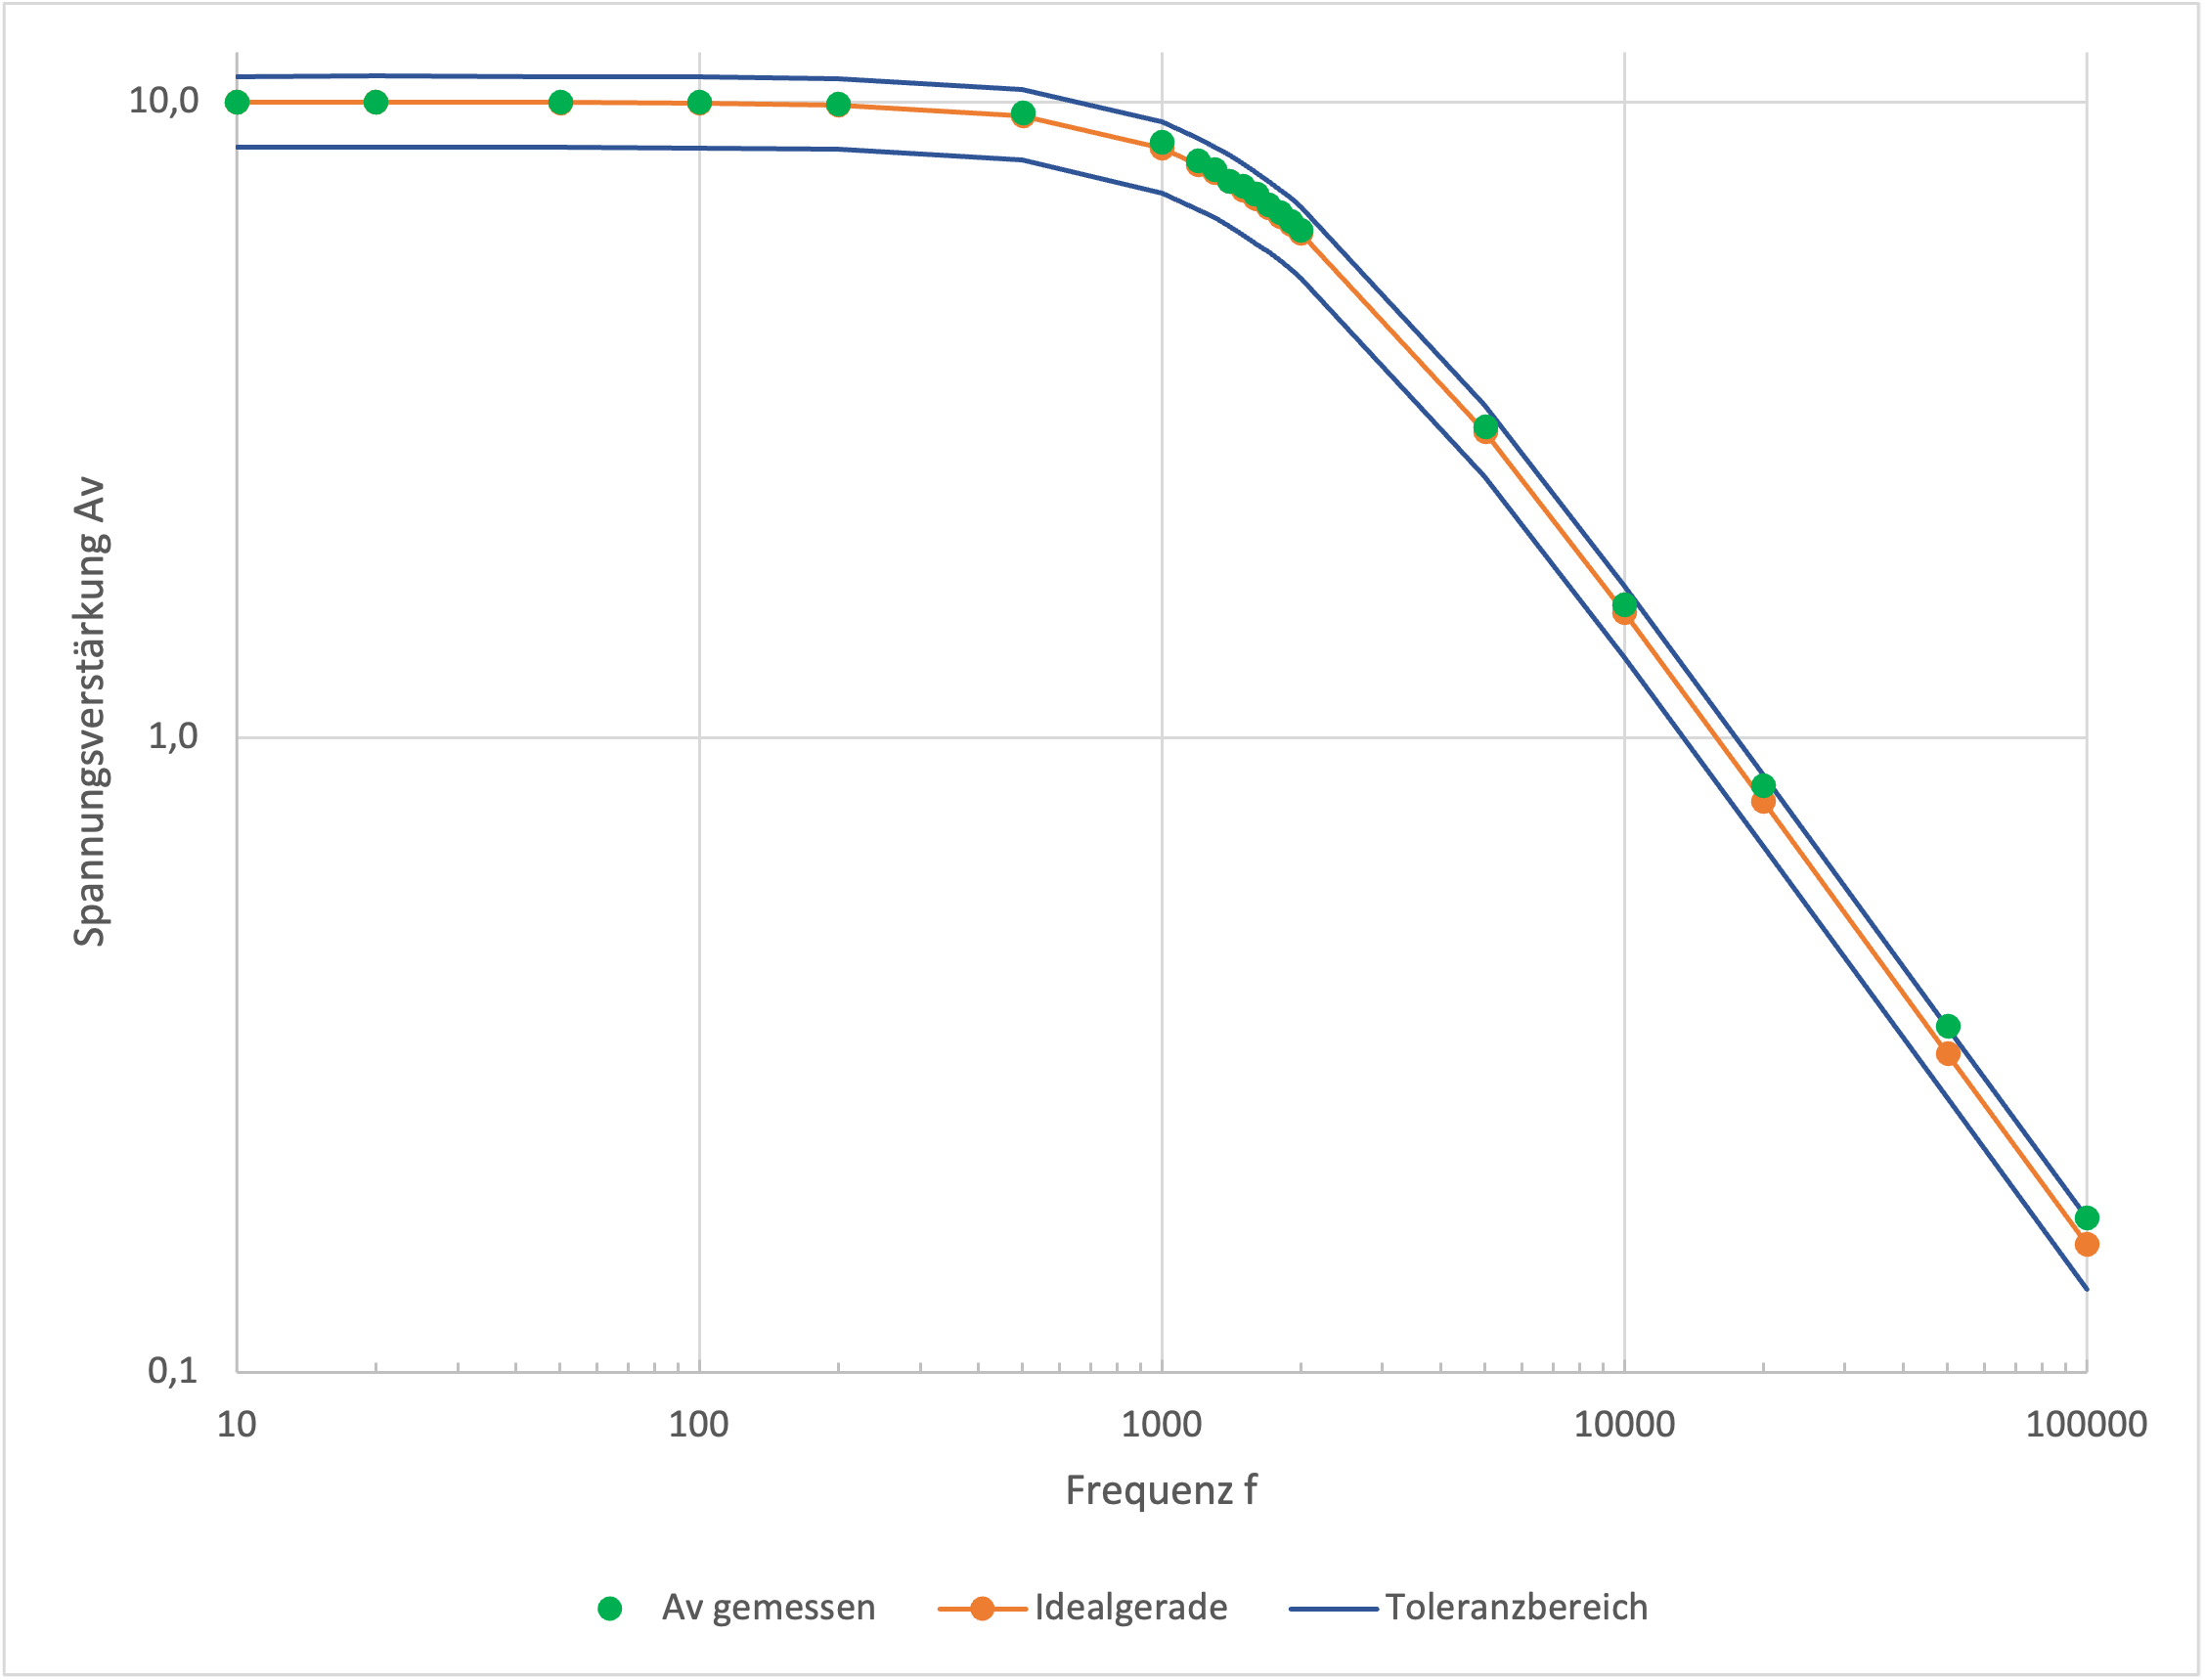
\includegraphics[height=8cm]{images/Versuch6/Graph_Spannungsverstaerkung.png} 
    \caption{Graph}
    \label{fig: Graph}
\end{figure}

\subsection{Fehlerrechnung}

$\frac{\Delta R_1}{R_1} = \frac{\Delta R_2}{R_2} = 5\%$, $\frac{\Delta C}{C} = 10\%$ \par

FB1: $|A_V| = \frac{R_2}{R_1}$

\[
    \begin{aligned}
        \Delta |A_{V, worst}| & = |\frac{\partial A_V}{\partial R_1} \cdot \Delta R_1| +
        |\frac{\partial A_V}{\partial R_2} \cdot \Delta R_2| = |- \frac{R_2}{R_1^2} \cdot \Delta R_1|
        + |\frac{1}{R_1} \cdot \Delta R_2| = \frac{R_2}{R_1} \cdot \frac{\Delta R_1}{R_1} + 
        \frac{R_2}{R_1} \cdot \frac{\Delta R_2}{R_2} \\
        & = A_V \cdot (\frac{\Delta R_1}{R_1} + \frac{\Delta R_2}{R_2}) = 
        10 \cdot (5\% + 5\%) = 1
    \end{aligned}
\]

\[
    |\frac{\Delta A_V}{A_V}| = \frac{\Delta R_1}{R_1} + \frac{\Delta R_2}{R_2} = 10\%
\]

FB3: $|A_V| = \frac{1}{2 \pi f R_1 C}$

\[
    \begin{aligned}
        \Delta |A_{V, worst}| & = 
        |\frac{\partial A_V}{\partial R_1} \cdot \Delta R_1| + |\frac{\partial A_V}{\partial C} \cdot \Delta C| 
        = |-\frac{1}{2 \pi f R_1^2 C} \cdot \Delta R_1| +
        |-\frac{1}{2 \pi f R_1 C^2} \cdot \Delta C| \\
        & = \frac{1}{2 \pi f R_1 C} \cdot (\frac{\Delta R_1}{R_1} + \frac{\Delta C}{C}) 
        = A_V \cdot (\frac{\Delta R_1}{R_1} + \frac{\Delta C}{C}) = 
        A_V \cdot (5\% + 10\%) = A_V \cdot 15\%
    \end{aligned}
\]

\[
    |\frac{\Delta A_V}{A_V}| = 15\%
\]

\section{Messungen}
Man baut die Schaltung aus Abbildung \ref{fig: Schaltungsskizze} auf.
Für den Eingangssignal u\textsubscript{e} wird ein Sinussignal
(da nach Fourier jedes Signal aus Sinussignalen zusammengesetzt ist)
mit einer Amplitude von 2V (gemessen 1,94V) verwendet. 
Man misst die Ausgangsspannung u\textsubscript{a} in Abhängigkeit
der Frequenz f im 1:2:5 Muster. Die Frequenz wird von 10Hz bis 
100kHz variiert. Die Eingangsspannung u\textsubscript{e} beträgt
1,94V. Die Messwerte sind in der folgenden Tabelle aufgelistet:

\begin{figure}[H]
    \centering
    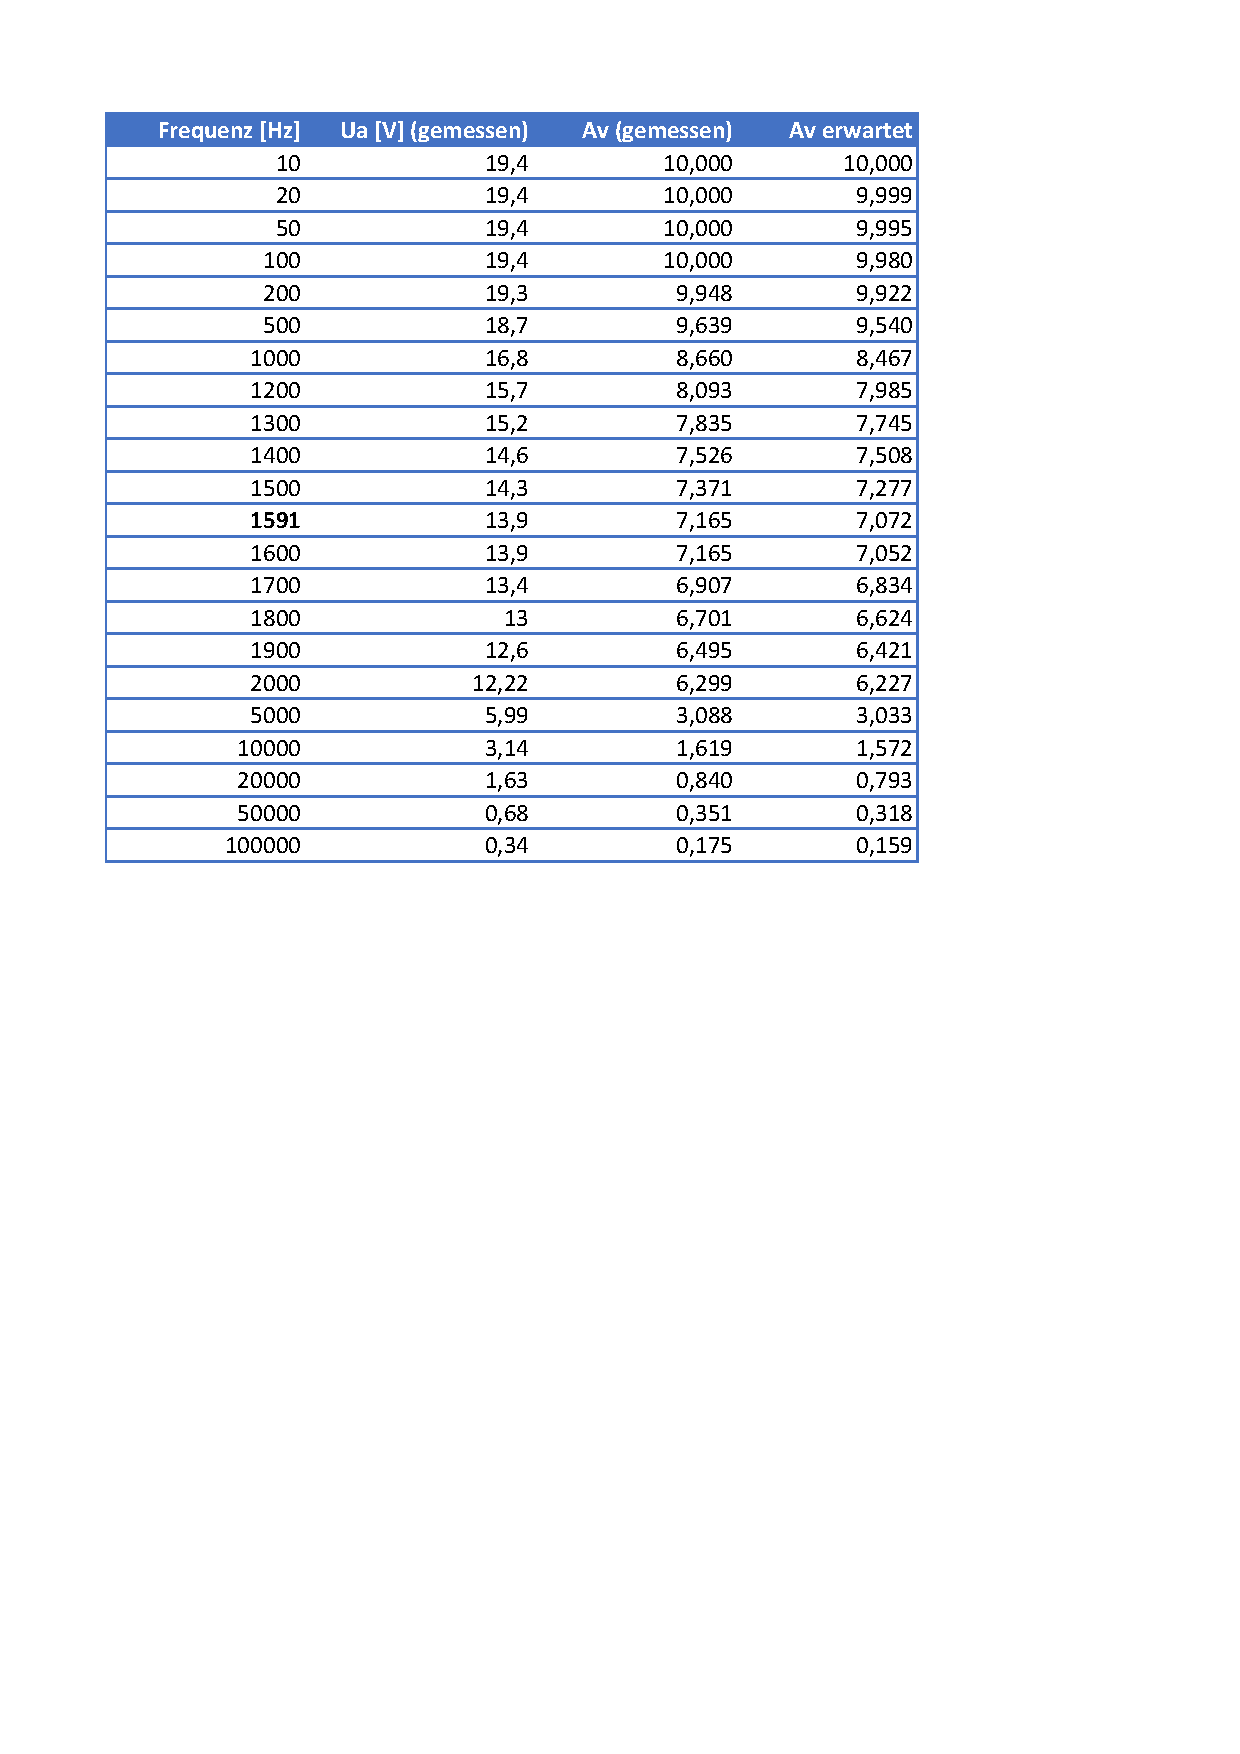
\includegraphics[height=10cm]{images/Versuch6/Tabelle.pdf} 
    \caption{Messwerte}
    \label{fig: Messwerte}
\end{figure}

\section{Auswertung}
Die Verstärkung sinkt um $\sqrt{2}$ ($\frac{10V}{\sqrt{2}} = 7,071V$) bei 1520Hz.
Differenz (absolut): $1591,549Hz - 1520Hz = 71,549Hz$
Differenz (prozentual): $\frac{71,549}{1591,549} = 4,49\%$

Die Verstärkung erreicht den Wert 1 bei der Transitfrequenz. Diese
beträgt (gemessen) 16200Hz.

Rechnerisch: 
\[
    \frac{1}{\sqrt{4 \pi^2 f^2 C^2 R_1^2 + (\frac{R_1}{R_2})}} = 1 \rightarrow f = 15835,72Hz
\]

Alle gemessenen Werte liegen innerhalb des Toleranzbandes.
Es ist zu erwarten, dass alle gemessenen Werte innerhalb der 
Fehlergrenzen liegen, denn der berechnete fehler ist der 
worst case Fehler.